\documentclass[conference]{IEEEtran}
\IEEEoverridecommandlockouts

\usepackage{graphicx}
\usepackage{hyperref}
\usepackage{amsmath}
\usepackage{float}

\begin{document}

\title{GetClasses: An Object-Oriented Transactional Platform for Online Tutoring}

\author{
    \IEEEauthorblockN{Jhon~Gonzalez}
    \IEEEauthorblockA{Student of Computer Engineering\\
    Universidad Distrital Francisco Jos\'e de Caldas\\
    Email: jjgonzalezc@udistrital.edu.co}
    \IEEEauthorblockA{code: 20251020087} 
    \and
    
    \IEEEauthorblockN{Alejandro~Escobar}
    \IEEEauthorblockA{Student of Computer Engineering\\
    Universidad Distrital Francisco Jos\'e de Caldas\\
    Email: aescobarb@udistrital.edu.co}
    \IEEEauthorblockA{code: 20251020094} 
   
    \\\\[-0.8em]
    
        \IEEEauthorblockN{Sebastián~Zambrano}
        \IEEEauthorblockA{Student of Computer Engineering\\
        Universidad Distrital Francisco Jos\'e de Caldas\\
        Email: szambranoh@udistrital.edu.co}
    \IEEEauthorblockA{code: 20251020102} 
    
}




\maketitle

\begin{abstract}
Online education platforms have become essential in providing accessible and personalized learning experiences. This paper introduces GetClasses, a transactional application that connects students with tutors in a secure and intuitive environment. The system applies object-oriented programming (OOP) principles and a layered architecture implemented in JavaFX. Results show a functional prototype with integrated scheduling, communication, and review modules, validating the design’s scalability and maintainability.
\end{abstract}

\begin{IEEEkeywords}
Object-Oriented Programming, Java, SOLID, Layered Architecture, JavaFX, Software Engineering, Online Learning
\end{IEEEkeywords}

\section{Introduction}
Online learning has become a major trend in recent years, requiring systems capable of connecting learners and educators efficiently and safely. Previous solutions, such as online tutoring platforms and learning management systems, often face challenges with integration, user experience, and reliability. Systems like Coursera and Udemy provide broad learning content but lack personalized tutor-student interaction and real-time scheduling. GetClasses addresses this gap by offering a transactional platform where tutors and students can interact, schedule sessions, make payments, and exchange feedback within a unified system.

The GetClasses project was developed as part of the Object-Oriented Programming course at Universidad Distrital Francisco Jos\'e de Caldas. It leverages modern software engineering practices, including UML modeling, SOLID principles, and layered architecture, to ensure clear separation of concerns, maintainability, and scalability. The project aims to demonstrate how OOP-based architectures can produce modular and robust educational software.

\section{Methods and Materials}
The project design follows a layered architecture consisting of three main layers: presentation, business logic, and persistence. The presentation layer uses JavaFX for GUI implementation, offering a responsive interface that allows users to register, search tutors, and manage sessions. The business logic layer implements system rules, ensuring that each transaction, schedule, and interaction follows the designed workflow. The persistence layer handles data storage through file-based mechanisms, later extendable to database integration.

\begin{figure}[H]
    \centering
    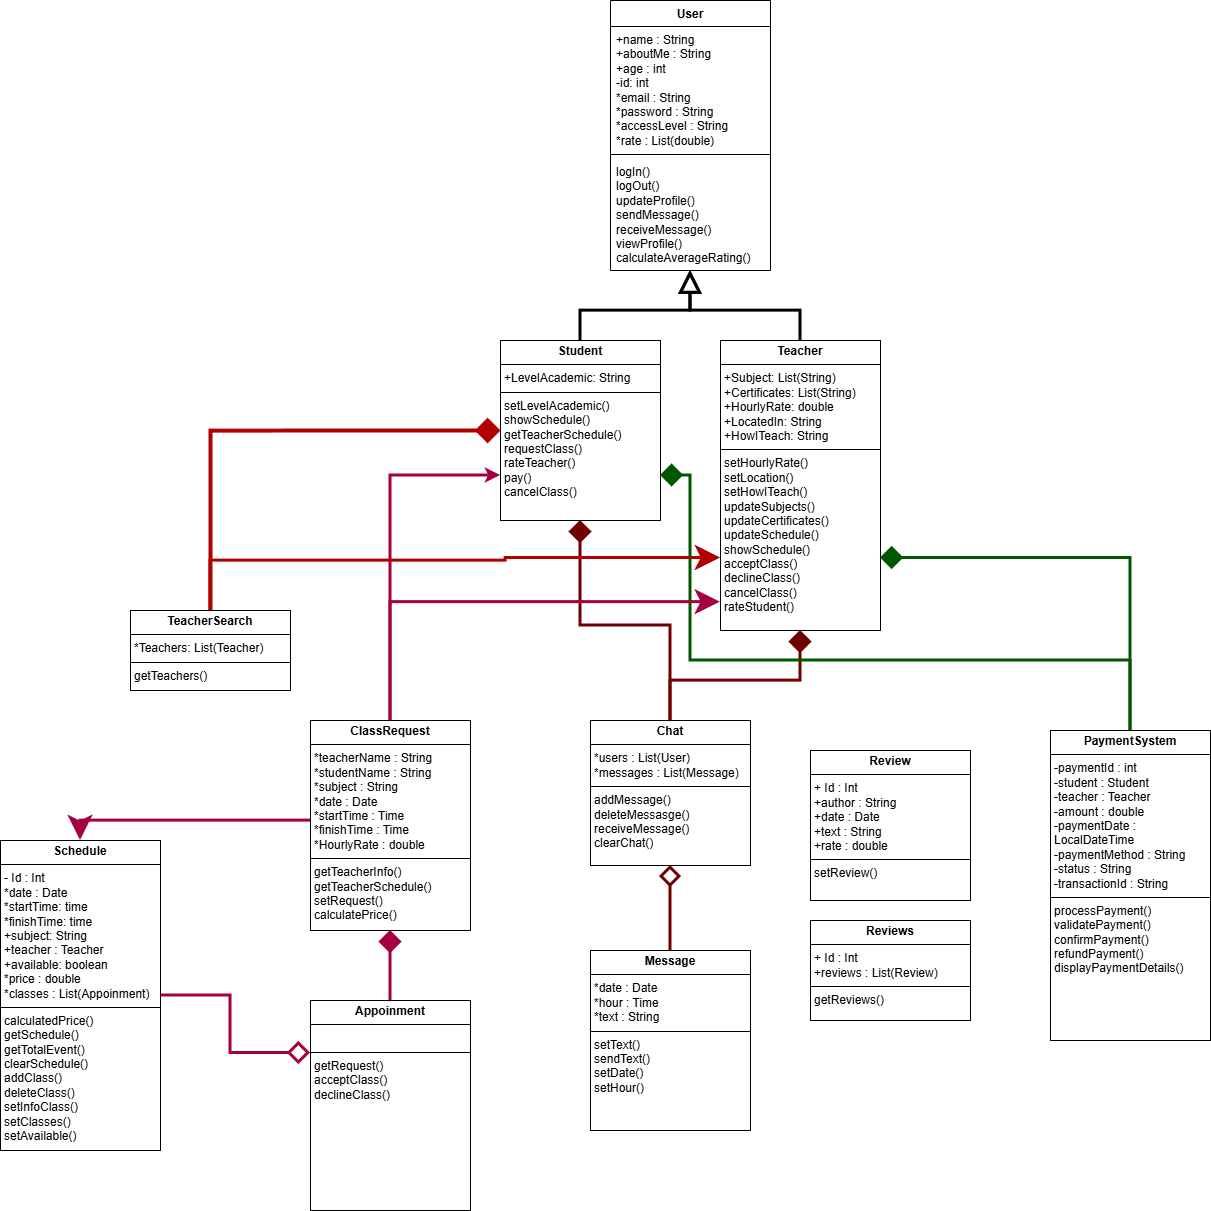
\includegraphics[width=0.45\textwidth]{UML.png}
    \caption{UML diagram showing inheritance and interactions among system entities.}
    \label{fig:uml}
\end{figure}

The UML class diagram (Fig.~\ref{fig:uml}) defines the system structure, with a base class \texttt{User} and specialized subclasses \texttt{StudentUser}, \texttt{TutorUser}, and \texttt{AdminUser}. Inheritance, polymorphism, and encapsulation are central to the design. The \texttt{User} class contains shared attributes (id, name, email, password) and methods (login, logout), while subclasses extend these with specific behaviors, such as class booking for students or availability management for tutors.



The GetClasses system integrates key OOP principles: encapsulation ensures secure attribute management; inheritance promotes code reuse; and polymorphism enables flexible interactions between components. SOLID principles guide the class responsibilities, reducing coupling and improving cohesion. CRC cards and user stories were used to align requirements and design decisions.

\section{Results and Discussion}
The first version of GetClasses provides full functionality across its core modules: registration, profile management, scheduling, chat, payment simulation, and review. Unit tests validated the correct behavior of user registration, tutor availability, and booking transactions. Integration tests confirmed interaction between modules without data loss.

Performance metrics show that typical queries (e.g., searching for tutors by subject or rate) execute in under three seconds. Usability evaluations confirmed an intuitive interface and smooth navigation. Table~\ref{tab:results} summarizes the main test outcomes.

\begin{table}[H]
\centering
\caption{Summary of functional testing results}
\resizebox{0.5\textwidth}{!}{
\begin{tabular}{|l|c|c|}
\hline
\textbf{Test Module} & \textbf{Status} & \textbf{Execution Time (s)} \\
\hline
Registration & In Progress  & 1.8 \\
\hline
Review System & In Progress  & 1.9 \\
\hline
Scheduling & In Progress  & 2.5 \\
\hline
Chat Module & Pending  & 2.0 \\
\hline
Payment Simulation & Pending  & 2.7 \\
\hline

\end{tabular}
}
\label{tab:results}
\end{table}


The prototype was validated by end users who provided feedback on usability and system responsiveness. Compared with traditional online tutoring platforms, GetClasses presents a more cohesive user flow and modular design, facilitating future updates and feature additions such as group sessions or advanced analytics.

\section{Conclusions}
This paper presented GetClasses, an object-oriented transactional platform that demonstrates the application of key OOP principles in real-world software. The system integrates design artifacts such as UML diagrams, CRC cards, and user stories, resulting in a modular, maintainable, and scalable solution. The use of layered architecture and SOLID principles ensures clear separation of responsibilities and system extensibility.

Future work includes implementing database persistence, adding AI-driven tutor matching, and deploying the system to a web environment. This project serves as an educational example of structured software design and development following IEEE documentation standards.

\section*{Acknowledgments}
The authors acknowledge the guidance of Eng. Carlos Andr\'es Sierra, M.Sc., during the Object-Oriented Programming course at Universidad Distrital Francisco Jos\'e de Caldas.

\begin{thebibliography}{00}
\bibitem{b1} I. Sommerville, \textit{Software Engineering}, 10th ed., Pearson, 2015.
\bibitem{b2} K. Beck and M. Fowler, \textit{Planning Extreme Programming}, Addison-Wesley, 2000.
\bibitem{b3} S. W. Ambler, \textit{Agile Modeling: UML Diagrams and Class Design}, AgileModeling.com, 2023.
\bibitem{b4} IEEE Standards Association, \textit{Guide to Software Design Documentation (IEEE 1016-2020)}, 2023.
\bibitem{b5} P. Coad and E. Yourdon, \textit{Object-Oriented Design}, Prentice Hall, 1991.
\bibitem{b6} Overleaf, \textit{LaTeX tutorial: Learn LaTeX step by step}, 2024.
\bibitem{b7} Visual Paradigm, \textit{CRC Cards Tutorial and Examples}, 2023.
\end{thebibliography}

\end{document}